\documentclass[landscape]{article}
\usepackage[pdftex]{graphicx}
\pagestyle{empty}
\oddsidemargin  -0.5 in
\evensidemargin -0.5 in
\headheight     0 in
\topmargin      -1 in
\textheight     7.7 in
\textwidth      10 in
\begin{document}
\huge
\renewcommand{\labelitemi}{-}
\setlength{\parindent}{0 cm}

\mbox{ }

\vfill

\mbox{ }

\vfill

\begin{center}
  Bounding the Trigger Inefficiency for $\Upsilon(1,2,3S)$

  \vfill

  Jim Pivarski
\end{center}

\vfill

\mbox{ }

\vfill

\pagebreak

\mbox{ }

\vfill

First cut in any analysis: the trigger

\vfill

Problem: only events which {\it pass} the trigger can be compared with
data

\vfill

My trigger lines: ``Hadron'' OR ``RadTau'' OR ``ElTrack''

\vfill

MC efficiency for these lines is 99.5\% (nicely bounded above)

\vfill

Is the MC generating {\it too few} untriggered events?

\vfill

\pagebreak

\mbox{ }

\vfill

\begin{center}
  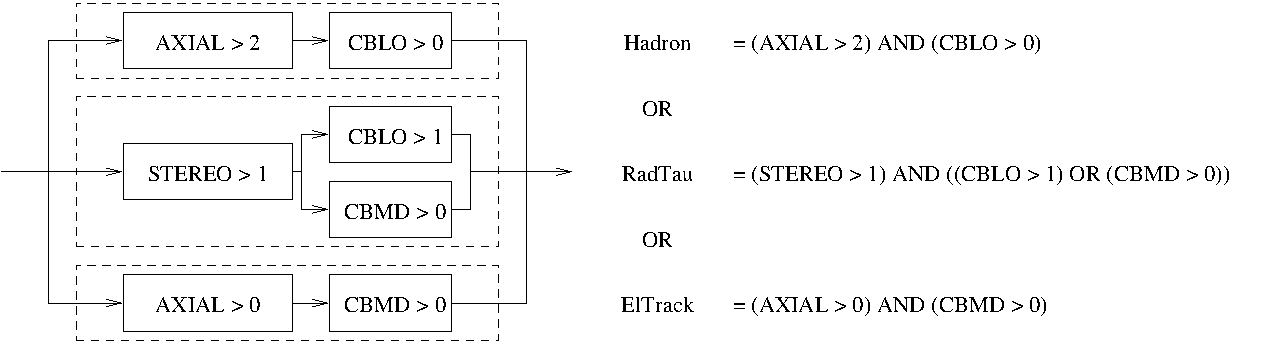
\includegraphics[width=\linewidth]{triggercuts.pdf}
\end{center}

\vfill

Trigger depends on four variables: $\begin{array}{c} \\ \underbrace{\mbox{\#AXIAL, \#STEREO,}} \\ \mbox{DR track counting} \end{array} \begin{array}{c} \\ \underbrace{\mbox{\#CBLO, \#CBMD}} \\ \mbox{CC cluster counting} \end{array}$

\vfill

\renewcommand{\labelitemi}{}
\begin{itemize}

  \item {STEP 1: Check CC cluster counting with ``TwoTrack'' trigger}

  \item {STEP 2: Quantify relevance of trigger track efficiency with toy MC}

  \item {STEP 3.1: Check MC track distribution with 2S to 1S cascade}

  \item {STEP 3.2: Quantify uncertainty in track distribution with toy MC}

  \item {STEP 3.3: Fill a loophole in this argument}

\end{itemize}
\renewcommand{\labelitemi}{-}

\vfill

\pagebreak

\vspace{1 cm}

{\bf STEP 1: Check CC cluster counting with ``TwoTrack'' trigger}

\vfill

P($\Upsilon$ passes trigger $|$ TwoTrack) = P(event passes trigger $|$ TwoTrack and event is $\Upsilon$)

\vfill

These cuts guarantee negligible backgrounds and no lower bounds on CC quantities:

\vspace{0.5 cm}

%%%%%%%%%%% charged energy cut reduces efficiency from 96% to 81%
\begin{center}
  \begin{tabular}{l l}
    data: TwoTrack trigger & \hspace{-0.4 cm} AND analysis cuts AND charged energy $>$ 35\% COM \\
    & \hspace{-0.4 cm} AND continuum-subtraction
  \end{tabular}

  \medskip
  \begin{tabular}{l}
    MC: TwoTrack trigger AND analysis cuts AND charged energy $>$ 35\% COM
  \end{tabular}
\end{center}

\vfill

P(passes ``Hadron'' OR ``RadTau'' OR ``ElTrack'' $|$ all those cuts):

\begin{center}
  \renewcommand{\arraystretch}{1.25}
  \begin{tabular}{c c c c}
  \mbox{\hspace{4 cm}} & \mbox{\hspace{2 cm}} $\Upsilon(1S)$ \mbox{\hspace{2 cm}} & \mbox{\hspace{2 cm}} $\Upsilon(2S)$ \mbox{\hspace{2 cm}} & \mbox{\hspace{2 cm}} $\Upsilon(3S)$ \mbox{\hspace{2 cm}} \\\hline
  data & 99.97\% & 99.48\% & 99.51\% \\
  MC & 99.83\% & 99.86\% & 99.86\% \\
  diff & 0.14\% & 0.38\% & 0.35\% \\
  & $\pm$0.20\% & $\pm$0.31\% & $\pm$1.00\%
  \end{tabular}
\end{center}

\pagebreak

\vspace{1 cm}

{\bf STEP 2: Quantify relevance of trigger track efficiency with toy MC}

\vfill

Assuming MC has the right charged particle multiplicity (and that this
is well represented by the number of quality tracks), how much does
trigger track efficiency/overcounting matter?

\vfill

Toy MC:
\begin{enumerate}

  \item pick a random \#tracks from the full MC's \#tracks distribution

  \item for this \#tracks, pick a random \#CBLO, \#CBMD (2-d distributions from full MC)

  \item for this \#tracks, pick a random \#AXIAL (same way)

  \item for this \#AXIAL, pick a random \#STEREO (same way)

  \item do this 100,000 times and calculate trigger efficiency

\end{enumerate}

\vfill

\begin{center}
  \renewcommand{\arraystretch}{1.25}
  \begin{tabular}{p{12 cm} c c c}
  & \mbox{\hspace{0.5 cm}} $\Upsilon(1S)$ \mbox{\hspace{0.5 cm}} & \mbox{\hspace{0.5 cm}} $\Upsilon(2S)$ \mbox{\hspace{0.5 cm}} & \mbox{\hspace{0.5 cm}} $\Upsilon(3S)$ \mbox{\hspace{0.5 cm}} \\\hline
  Full MC & 99.68\% & 99.44\% & 99.50\% \\
  Toy MC (baseline) & 99.67\% & 99.54\% & 99.64\% \\
  Get \#AXIAL, \#STEREO from data & 99.56\% & 99.42\% & 99.49\% \\
  Set \#STEREO = \#AXIAL & 99.79\% & & \\
  Set \#STEREO = \#AXIAL = \#tracks & 99.43\% & & \\
  \end{tabular}
\end{center}
\begin{flushright} ($\pm$0.03\% in all cases) \end{flushright}

\vfill

\pagebreak

\vspace{1 cm}

{\bf STEP 2: Quantify relevance of trigger track efficiency with toy MC}

\vfill

Assuming MC has the right charged particle multiplicity (and that this
is well represented by the number of quality tracks), how much does
trigger track efficiency/overcounting matter?

\vfill

Toy MC:
\begin{enumerate}

  \item pick a random \#tracks from the full MC's \#tracks distribution

  \item for this \#tracks, pick a random \#CBLO, \#CBMD (2-d distributions from full MC)

  \item for this \#tracks, pick a random \#AXIAL (same way)

  \item for this \#AXIAL, pick a random \#STEREO (same way)

  \item do this 100,000 times and calculate trigger efficiency

\end{enumerate}

\vfill

\begin{center}
  \renewcommand{\arraystretch}{1.25}
  \begin{tabular}{p{12 cm} c c c}
  & \mbox{\hspace{0.5 cm}} $\Upsilon(1S)$ \mbox{\hspace{0.5 cm}} & \mbox{\hspace{0.5 cm}} $\Upsilon(2S)$ \mbox{\hspace{0.5 cm}} & \mbox{\hspace{0.5 cm}} $\Upsilon(3S)$ \mbox{\hspace{0.5 cm}} \\\hline
  Full MC & 0.01\% & -0.10\% & -0.14\% \\
  Toy MC (baseline) & 0\% & 0\% & 0\% \\
  Get \#AXIAL, \#STEREO from data & -0.11\% & -0.12\% & -0.15\% \\
  Set \#STEREO = \#AXIAL & 0.12\% & & \\
  Set \#STEREO = \#AXIAL = \#tracks & -0.24\% & & \\
  \end{tabular}
\end{center}
\begin{flushright} ($\pm$0.03\% in all cases) \end{flushright}

\vfill

\pagebreak

\vspace{1 cm}

{\bf STEP 3.1: Check MC track distribution with 2S to 1S cascade}

\vfill

Verify the assumtion: ``MC has the right charged particle
multiplicity.''  (We continue to assume that track distribution
represents charged multiplicity.)

\vfill

$\Upsilon(2S) \to \Upsilon(1S) \underbrace{\pi^+\pi^-}$

\hspace{5.5 cm} $\hookrightarrow$ satisfy TwoTrack requirement, L4, and ``quality tracks $\ge$ 2''

\begin{tabular}{p{0.5\linewidth} p{0.5\linewidth}}
  \begin{minipage}{\linewidth}

  \begin{enumerate}

    \item Get {\bf all} $\Upsilon(2S)$ events from tau subcollection with TwoTrack trigger

    \item Plot $\pi^+\pi^-$ missing mass distribution for each number of tracks

%%     \item Scale up wrong-sign combinations to match right-sign, using sideband

%%     \item Subtract $\Upsilon(1S)$ mass peak from combinatoric background

    \item Count number of $\Upsilon(1S)$ events in each peak

    \item Do exactly the same for $\Upsilon(2S)$ MC

    \item Plot number of $\Upsilon(1S)$ events per number of non-$\pi^+\pi^-$ tracks $\longrightarrow$ $\longrightarrow$ $\longrightarrow$ $\longrightarrow$

  \end{enumerate}

  \end{minipage} &
  \begin{minipage}{\linewidth} 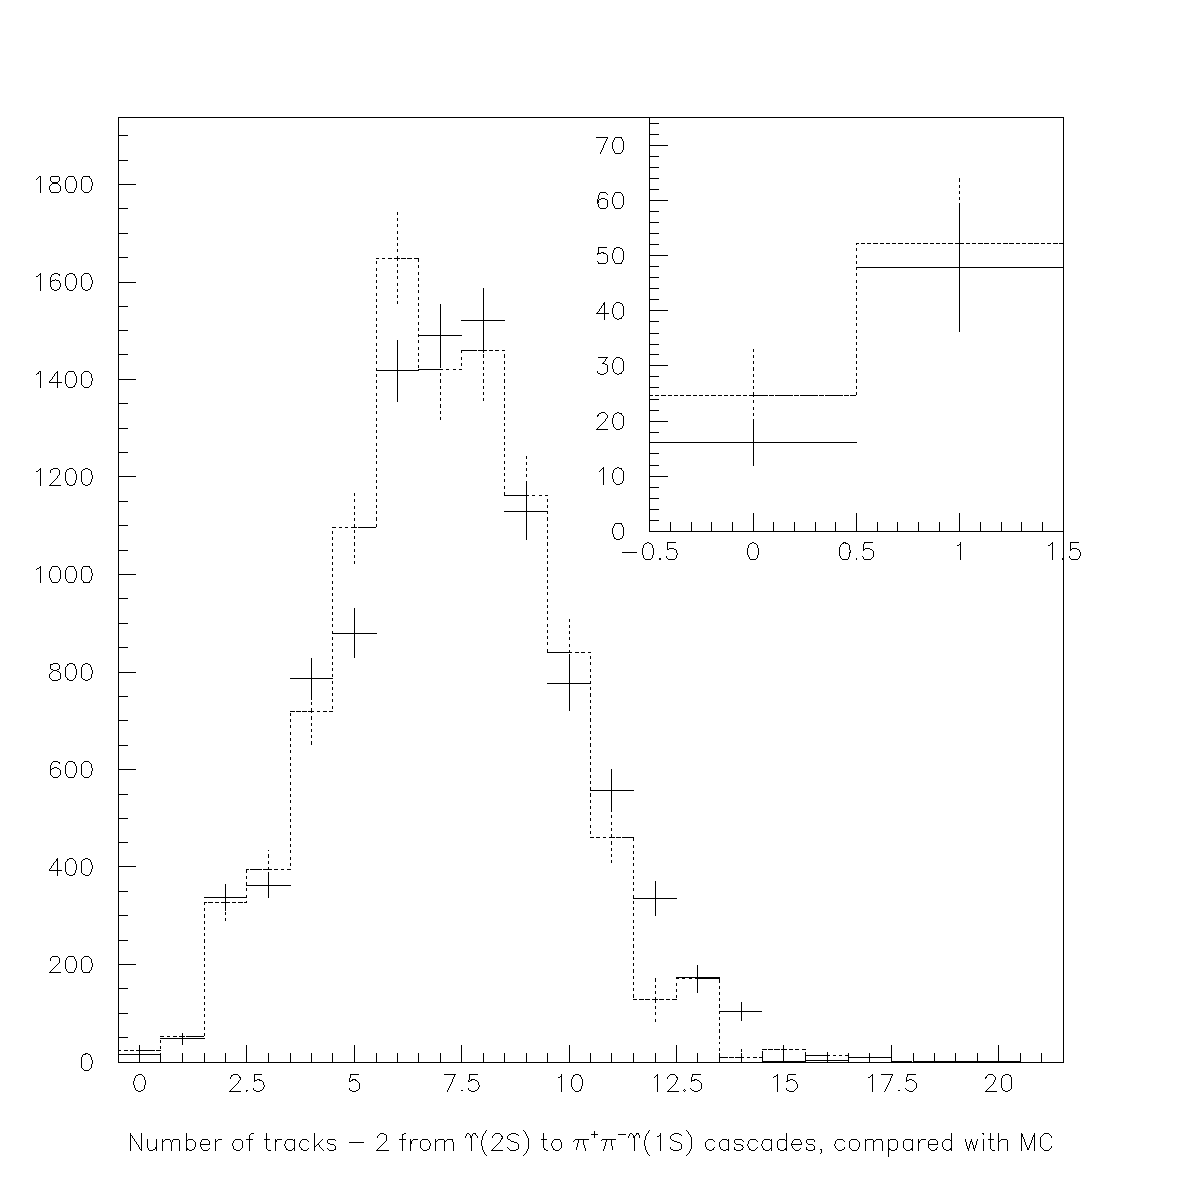
\includegraphics[width=\linewidth]{cascades_tracks_boost_tt.pdf} \end{minipage}
\end{tabular}

\pagebreak

\vspace{1 cm}

{\bf STEP 3.2: Quantify uncertainty in track distribution with toy MC}

\vfill

Instead of replacing the \#AXIAL and \#STEREO distributions, replace
\#tracks.

\vfill

This is how much the uncertainty in MC track distribution matters for
correct trigger efficiency.

\vfill

(For apples-to-apples, we must compare {\it boosted} data to {\it boosted} MC.)

\vfill

\begin{center}
  \renewcommand{\arraystretch}{1.25}
  \begin{tabular}{p{12 cm} c c c}
  & \mbox{\hspace{0.5 cm}} $\Upsilon(1S)$ \mbox{\hspace{0.5 cm}} & \mbox{\hspace{0.5 cm}} $\Upsilon(2S)$ \mbox{\hspace{0.5 cm}} & \mbox{\hspace{0.5 cm}} $\Upsilon(3S)$ \mbox{\hspace{0.5 cm}} \\\hline
  Full MC & 99.68\% & 99.44\% & 99.50\% \\
  Toy MC & 99.67\% & 99.54\% & 99.64\% \\
  with boosted MC tracks (baseline) & 99.58\% & & \\
  with boosted data tracks & 99.65\% & & \\
  same with 0-, 1-tracks raised 1$\sigma$ & 99.61\% & & \\
  same with 100 extra 0-track events & 99.35\% & & \\
  same with 200 extra 0-track events & 99.12\% & &
  \end{tabular}
\end{center}
\begin{flushright} (The 0-track bin had 20$\pm$9 events, so 100 is way too many.) \end{flushright}

\vfill

\pagebreak

\vspace{1 cm}

{\bf STEP 3.2: Quantify uncertainty in track distribution with toy MC}

\vfill

Instead of replacing the \#AXIAL and \#STEREO distributions, replace
\#tracks.

\vfill

This is how much the uncertainty in MC track distribution matters for
correct trigger efficiency.

\vfill

(For apples-to-apples, we must compare {\it boosted} data to {\it boosted} MC.)

\vfill

\begin{center}
  \renewcommand{\arraystretch}{1.25}
  \begin{tabular}{p{12 cm} c c c}
  & \mbox{\hspace{0.5 cm}} $\Upsilon(1S)$ \mbox{\hspace{0.5 cm}} & \mbox{\hspace{0.5 cm}} $\Upsilon(2S)$ \mbox{\hspace{0.5 cm}} & \mbox{\hspace{0.5 cm}} $\Upsilon(3S)$ \mbox{\hspace{0.5 cm}} \\\hline
  Full MC & 0.10\% & $-$ & $-$ \\
  Toy MC & 0.09\% & $-$ & $-$ \\
  with boosted MC tracks (baseline) & 0\% & & \\
  with boosted data tracks & 0.07\% & & \\
  same with 0-, 1-tracks raised 1$\sigma$ & 0.03\% & & \\
  same with 100 extra 0-track events & -0.23\% & & \\
  same with 200 extra 0-track events & -0.46\% & &
  \end{tabular}
\end{center}
\begin{flushright} (The 0-track bin had 20$\pm$9 events, so 100 is way too many.) \end{flushright}

\vfill

\pagebreak

\vspace{1 cm}

{\bf STEP 3.3: Fill a loophole in this argument}

\vfill

We assumed: ``number of quality tracks represents charged particle
multiplicity.''

\vfill

If MC generator overestimates number of charged particles and CLEOG
underestimates tracking efficiency, data and MC can have the same track
distribution while MC has too few trigger-failing events.

\begin{center}
  \begin{tabular}{p{0.35\linewidth} p{0.05\linewidth} p{0.35\linewidth}}
    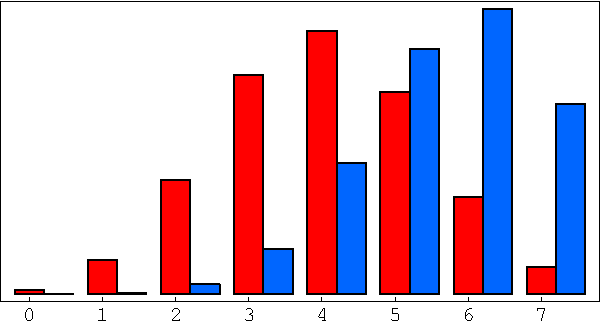
\includegraphics[width=\linewidth]{effcheck_datavmc1.pdf} & &
    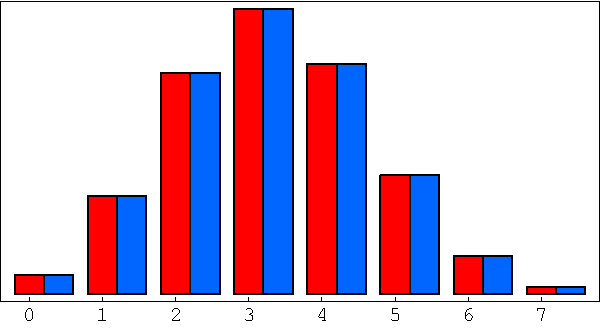
\includegraphics[width=\linewidth]{effcheck_datavmc2.pdf} \\
    \begin{center} \vspace{-1 cm} Number of Charged Particles \end{center} & &
    \begin{center} \vspace{-1 cm} Number of Quality Tracks \end{center}
  \end{tabular}
\end{center}

Technique \#1:  Put data track distribution AND data trigger distributions into toy MC

\begin{center}
  \renewcommand{\arraystretch}{1.25}
  \begin{tabular}{p{12 cm} c c c}
  & \mbox{\hspace{0.5 cm}} $\Upsilon(1S)$ \mbox{\hspace{0.5 cm}} & \mbox{\hspace{0.5 cm}} $\Upsilon(2S)$ \mbox{\hspace{0.5 cm}} & \mbox{\hspace{0.5 cm}} $\Upsilon(3S)$ \mbox{\hspace{0.5 cm}} \\\hline
  with boosted MC tracks (baseline) & 99.58\% & & \\
  with boosted data tracks and trigger & 99.47\% & & \\
  \end{tabular}
\end{center}

\vfill

\pagebreak

\vspace{1 cm}

{\bf STEP 3.3: Fill a loophole in this argument}

\vfill

We assumed: ``number of quality tracks represents charged particle
multiplicity.''

\vfill

If MC generator overestimates number of charged particles and CLEOG
underestimates tracking efficiency, data and MC can have the same track
distribution while MC has too few trigger-failing events.

\begin{center}
  \begin{tabular}{p{0.35\linewidth} p{0.05\linewidth} p{0.35\linewidth}}
    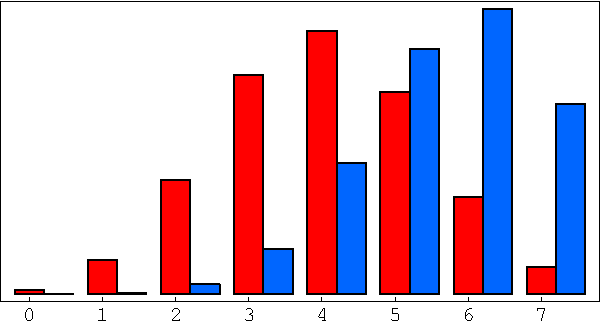
\includegraphics[width=\linewidth]{effcheck_datavmc1.pdf} & &
    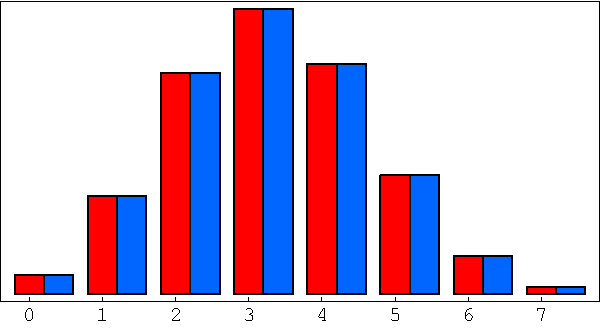
\includegraphics[width=\linewidth]{effcheck_datavmc2.pdf} \\
    \begin{center} \vspace{-1 cm} Number of Charged Particles \end{center} & &
    \begin{center} \vspace{-1 cm} Number of Quality Tracks \end{center}
  \end{tabular}
\end{center}

Technique \#1:  Put data track distribution AND data trigger distributions into toy MC

\begin{center}
  \renewcommand{\arraystretch}{1.25}
  \begin{tabular}{p{12 cm} c c c}
  & \mbox{\hspace{0.5 cm}} $\Upsilon(1S)$ \mbox{\hspace{0.5 cm}} & \mbox{\hspace{0.5 cm}} $\Upsilon(2S)$ \mbox{\hspace{0.5 cm}} & \mbox{\hspace{0.5 cm}} $\Upsilon(3S)$ \mbox{\hspace{0.5 cm}} \\\hline
  with boosted MC tracks (baseline) & 0\% & & \\
  with boosted data tracks and trigger & -0.11\% & & \\
  \end{tabular}
\end{center}

\vfill

\pagebreak

\vspace{1 cm}

{\bf STEP 3.3: Fill a loophole in this argument}

\vfill

Technique \#2:  Increase track-finding efficiency by the expected +2\% $\pm$1.5\%

\vfill

(I keep the number of generated particles fixed, but increase the tracking efficiency.)

\vfill

\vspace{4.5 cm}

\includegraphics[width=\linewidth, height=3.4 cm]{yellow.pdf}
\vspace{-4.5 cm}
\vspace{-0.4 cm}
\vspace{-4.05 cm}

\begin{center}
  \renewcommand{\arraystretch}{1.25}
  \begin{tabular}{p{12 cm} c c c}
  & \mbox{\hspace{0.5 cm}} $\Upsilon(1S)$ \mbox{\hspace{0.5 cm}} & \mbox{\hspace{0.5 cm}} $\Upsilon(2S)$ \mbox{\hspace{0.5 cm}} & \mbox{\hspace{0.5 cm}} $\Upsilon(3S)$ \mbox{\hspace{0.5 cm}} \\\hline
  Full MC           & 99.68\% & 99.44\% & 99.50\% \\
  Toy MC (baseline) & 99.67\% & 99.54\% & 99.64\% \\
  $+$5\%            & 99.76\% & & \\
  $+$2\% $+$ 1.5\%  & 99.71\% & 99.62\% & 99.72\% \\
  $+$2\%            & 99.69\% & 99.61\% & 99.67\% \\
  $+$2\% $-$ 1.5\%  & 99.69\% & 99.55\% & 99.68\% \\
  $-$2\%            & 99.69\% & & \\
  $-$10\%           & 99.58\% & & \\
  $-$20\%           & 99.33\% & & \\
  \end{tabular}
\end{center}

\vfill

$+n$\% is a simulated increase in MC tracking efficiency, obtained by
de-convolving the MC track distribution to first order in $n$\%.

\vfill

$-n$\% is a further decrease in MC tracking efficiency via an exact
convolution.

\pagebreak

\vspace{1 cm}

{\bf STEP 3.3: Fill a loophole in this argument}

\vfill

Technique \#2:  Increase track-finding efficiency by the expected +2\% $\pm$1.5\%

\vfill

(I keep the number of generated particles fixed, but increase the tracking efficiency.)

\vfill

\vspace{4.5 cm}

\includegraphics[width=\linewidth, height=3.4 cm]{yellow.pdf}
\vspace{-4.5 cm}
\vspace{-0.4 cm}
\vspace{-4.05 cm}

\begin{center}
  \renewcommand{\arraystretch}{1.25}
  \begin{tabular}{p{12 cm} c c c}
  & \mbox{\hspace{0.5 cm}} $\Upsilon(1S)$ \mbox{\hspace{0.5 cm}} & \mbox{\hspace{0.5 cm}} $\Upsilon(2S)$ \mbox{\hspace{0.5 cm}} & \mbox{\hspace{0.5 cm}} $\Upsilon(3S)$ \mbox{\hspace{0.5 cm}} \\\hline
  Full MC           &  0.01\% & -0.10\% & -0.14\% \\
  Toy MC (baseline) &  0\%    &  0\%    &  0\% \\
  $+$5\%            &  0.09\% & & \\
  $+$2\% $+$ 1.5\%  &  0.04\% &  0.08\% &  0.08\% \\
  $+$2\%            &  0.02\% &  0.07\% &  0.03\% \\
  $+$2\% $-$ 1.5\%  &  0.02\% &  0.01\% &  0.04\% \\
  $-$2\%            &  0.02\% & & \\
  $-$10\%           & -0.09\% & & \\
  $-$20\%           & -0.34\% & & \\
  \end{tabular}
\end{center}

\vfill

$+n$\% is a simulated increase in MC tracking efficiency, obtained by
de-convolving the MC track distribution to first order in $n$\%.

\vfill

$-n$\% is a further decrease in MC tracking efficiency via an exact
convolution.

\pagebreak

Summary of trigger efficiency systematic errors:

\begin{center}
  \renewcommand{\arraystretch}{1.25}
  \begin{tabular}{p{13 cm} c c c}
    & \mbox{\hspace{0.5 cm}} $\Upsilon(1S)$ \mbox{\hspace{0.5 cm}} & \mbox{\hspace{0.5 cm}} $\Upsilon(2S)$ \mbox{\hspace{0.5 cm}} & \mbox{\hspace{0.5 cm}} $\Upsilon(3S)$ \mbox{\hspace{0.5 cm}} \\\hline
    CC cluster counting (STEP 1) & 0.20\% & 0.31\% & 0.31\% \\
    trigger track efficiency (STEP 2) & 0.11\% & 0.12\% & 0.15\% \\
    reconstructed track distribution (STEP 3.2) & 0.08\% & 0.08\% & 0.08\% \\
    reconstructed track efficiency (STEP 3.3) & 0.11\% & 0.11\% & 0.11\% \\\hline\hline
    & 0.27\% & 0.36\% & 0.37\% \\
  \end{tabular}
\end{center}

\vfill

\begin{tabular}{p{0.5\linewidth} c p{0.4\linewidth}}
  \begin{minipage}{\linewidth}
    What could still go wrong?

    \bigskip
    
    Cascades study could miss events with:

    \begin{itemize}

      \item visible energy $>$ 20\% $\Upsilon(1S)$ mass,

      \item CC energy $<$ 90\% $\Upsilon(1S)$ mass,

\begin{center} OR \end{center}

      \item biggest shower $<$ 90\% $\Upsilon(1S)$ mass / 2

    \end{itemize}

  \end{minipage} & \mbox{\hspace{0.5 cm}} &
  \begin{minipage}{\linewidth}
    \begin{center}
      Zero-track events ($\sim\frac{1}{2}$ signal)

      \medskip

      \mbox{\hspace{0.5 cm}} 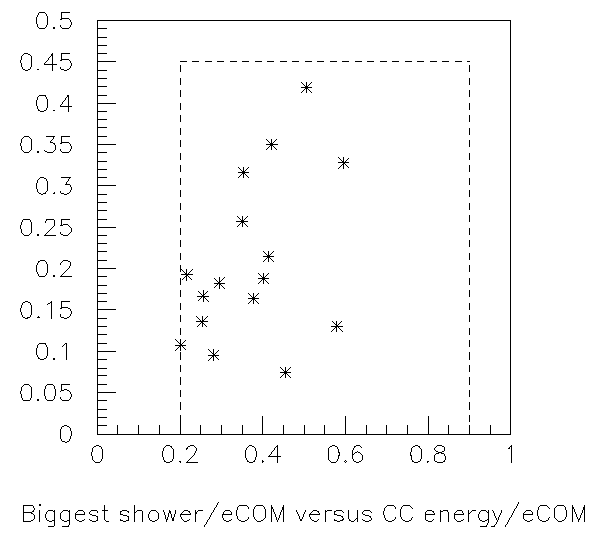
\includegraphics[width=0.9\linewidth]{cascade_still_missing3_tt.pdf}

      \medskip

      (Need about 100 unseen events)
    \end{center}
  \end{minipage}
\end{tabular}




\end{document}
